\section{The MXFP4 source is discrete}
\label{sec:theory}

We normalize each column $j$ of an MXFP4 matrix by a power of two, $\tilde w_{ij}=w_{ij}/2^{p_j}$. Each normalized
weight is still an E2M1 value times a power of two, and pooled over columns the values form a discrete source with
small support. We compute its memoryless distortion--rate function under squared error with
Blahut--Arimoto~\citep{blahut1972,arimoto1972} on the pooled values of all weights in \final{SRC-N} matrices (two
experts in each of 11 layers). The reconstruction points are free. Starting from the source values and their
midpoints, each point moves after every Blahut--Arimoto step to the centroid of the source values mapped to it, and
each slope is iterated until the Lagrangian changes by less than $10^{-13}$. Fixing the points at the source values
and midpoints raises the distortion at 3 bits by only \final{BA-GRIDGAP}. Every computed point is achievable, so the
lower envelope of the two computations is an upper estimate of the memoryless distortion--rate function. We compare
this estimate with $D_G(R)=\sigma^2 2^{-2R}$, the distortion--rate function of a Gaussian source of the same variance.
Among sources of variance $\sigma^2$, the
Gaussian has the largest $D(R)$~\citep{cover2006}, whereas a discrete source with entropy $H$ has $D(R)=0$ for
$R\ge H$. A random rotation leaves the vector source's $D(R)$ unchanged, but it moves the discreteness into the joint
distribution of each 128-dimensional block. Coders such as EXL3 model the rotated coordinates as i.i.d.\ Gaussian, and
their codebooks are designed for $D_G(R)$. EXL3's trellis comes within about \final{EXL3-GAUSS} of $D_G(R)$ on
Gaussian tiles, and on DeepSeek's own weights after EXL3's rotation its error stays at \final{EXL3-ROT-X} $D_G(R)$
(\cref{fig:rd}a). We do not prove that no rotation-based coder can do better, but GRAFT's codebook is built for the
discrete source, which these coders do not model.

For a synthetic MXFP4 source with entropy \final{TOY-ENTROPY} bits, the ratio of its distortion--rate function to the
Gaussian one (reconstruction on the source values and their midpoints) is \final{TOY-R2}, \final{TOY-R25}, \final{TOY-R3} and \final{TOY-R35} at 2, 2.5, 3 and 3.5 bits. For
DeepSeek-V4.1-Flash's weights in GRAFT's power-of-two column domain (entropy \final{DS-ENTROPY} bits), the ratio is
\final{DS-BOUND3} at 3 bits and \final{DS-BOUND35} at 3.5. Three consequences follow for GRAFT.
(i) The gain grows as the rate approaches the entropy, so 2.5--3.5 bits is the useful band for an MXFP4 source,
and rate is worth more than it is for a Gaussian source. (ii) Scales must be commensurate with the grid. A
non-power-of-two column scale moves the column off the shared grid, and on DeepSeek such free scales leave
\final{FREE-SCALES} more error than powers of two (\cref{sec:method}). (iii) The optimal reproduction distribution puts its mass on the modal grid points and about \final{ZERO-MASS} near zero, so an E2M1 alphabet suffices (\cref{fig:qtail}).

The source is also close to memoryless in our measurements, which motivates the i.i.d.\ reference. On twelve DeepSeek
matrices the codes carry \final{CODE-H} bits each. Conditioning on the previous code along the input dimension lowers
this by \final{CODE-K1} bits, and conditioning on the previous two codes by \final{CODE-K2}. The neighbouring column's
code does not lower it at all, and the block's scale lowers it by at most \final{CODE-SCALE}, a
dependence that per-column scales and per-block flags capture. We also found no useful shared linear subspace
across experts, since the leading directions of half of a layer's experts capture only the isotropic share of the other
half's weight energy (\final{LOWRANK} against \final{LOWRANK-ISO} at rank 1,024 of 5,120).

\begin{figure*}[t]
\centering
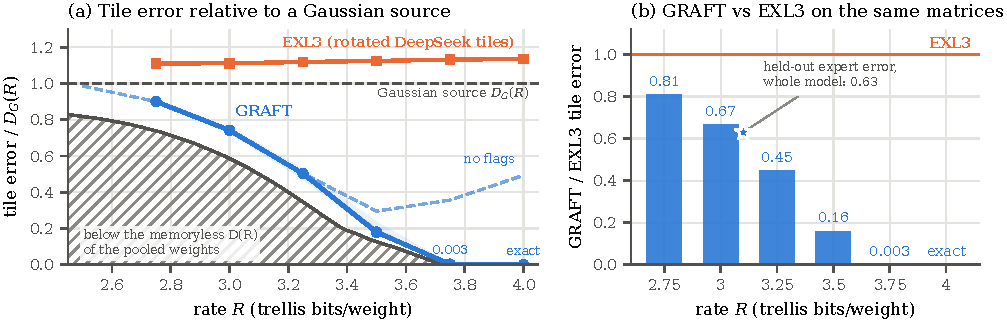
\includegraphics[width=\textwidth]{figures/fig_rd}
\caption{GRAFT's tile error relative to a Gaussian source. (a) Raw-tile error divided by $D_G(R)=2^{-2R}$, the
distortion--rate function of a Gaussian source of the same variance. GRAFT (solid; block flags where they pay for their
bit, per-matrix widths, tail band 0) on every routed-expert matrix of 11 layers of DeepSeek-V4.1-Flash
(\final{MX11-N} matrices, 96 seeded tiles each; median, interquartile and 10--90\% bands) reaches \final{GRAFT-GAUSS3}
at 3 bits, \final{GRAFT-GAUSS35} at 3.5 and \final{GRAFT-GAUSS375} at 3.75, and at 4 bits it reproduces every sampled
tile of \final{EXACT4} of the matrices exactly. Dashed: the same codebook without flags on all 46,080 matrices. It
stops improving above 3.5 bits (\final{NOFLAG-GAUSS4} at 4), because blocks whose MX scale is an octave below their
column's need the halved grid, which only the flags provide. Squares: EXL3's codebook on \final{ROT-N} of these
matrices after EXL3's rotation (\final{ROT-TILES} tiles each, median), at about \final{EXL3-ROT-X} $D_G(R)$; on
Gaussian tiles it comes within \final{EXL3-GAUSS} of $D_G(R)$. Hatched: below the memoryless distortion--rate
function of the pooled weights (entropy \final{DS-ENTROPY} bits), a reference for the per-matrix medians rather than a
bound for each matrix. The rate counts trellis bits only. (b) GRAFT's tile error relative to EXL3's on the same \final{ROT-N} matrices
(median of the per-matrix ratios); star: GRAFT's held-out expert error relative to EXL3 over the whole model at 3
bits.}
\label{fig:rd}
\end{figure*}
